\documentclass[main.tex]{subfiles}
\begin{document}



\section{Topologie in $\mathbb{R}^p$}
\label{sec:topologie-mathbbrp}

\begin{de}
  We gebruiken $B(x,\delta)$ als afkorting voor de volgende verzameling en noemen dit de \term{open bol} rond $x$ met straal $\delta$.
  \[ B(x,\delta) = \{ y \in \mathbb{R}^{p} \mid \|x-y\| < \delta \} \]
\end{de}

\begin{de}
  We gebruiken $B\interval{x}{\delta}$ als afkorting voor de volgende verzameling en noemen dit de \term{gesloten bol} rond $x$ met straal $\delta$.
  \[ B\interval{x}{\delta} = \{ y \in \mathbb{R}^{p} \mid \|x-y\| \le \delta \} \]
\end{de}

\begin{de}
  We noemen een deelverzameling $A$ van $\mathbb{R}^{+}$ \term{begrensd} als er een $M \in \mathbb{R}^{+}$ bestaat als volgt:
  \[ \forall x \in A:\ x \le M \]
\end{de}

\begin{de}
  We noemen een deelverzameling $A$ van $\mathbb{R}^{p}$ \term{open} als het volgende geldt:
  \[ \forall x\in A, \exists \delta \in \mathbb{R}_{0}^{+}, \forall y\in \mathbb{R}^{p}:\ \|y-x\| < \delta \Rightarrow y \in A \]
\end{de}

\begin{opm}
  Een deelverzameling $A$ van $\mathbb{R}^{p}$ is dus open als en slechts als er rond elk punt $x\in A$ een open bol kan gevonden worden die helemaal binnen $A$ ligt.
\extra{bewijs?}
\end{opm}

\begin{st}
  Equivalente definitie van open\\
  Zij $A$ een deelverzameling van $\mathbb{R}^{p}$, dan is $A$ open als en slechts er, voor elke $x\in A$ een $\delta\in\mathbb{R}_{0}^{+}$ bestaat zodat $B\interval{x}{\delta}$ volledig binnen $A$ ligt.

  \begin{proof}
    Bewijs van een equivalentie
    \begin{itemize}
    \item $\Rightarrow$\\
      Zij $A$ open en $x\in A$ willekeurig.
      Omdat $A$ open is bestaat er een $\epsilon \in \mathbb{R}_{0}^{+}$ zodat $B(x,\epsilon)$ binnen $A$ ligt.
      Kies nu $\delta = \frac{\epsilon}{2}$, dan ligt $B\interval{x}{\delta}$ binnen $B(x,\epsilon)$ en dus binnen $A$.
    \item $\Leftarrow$\\
      Kies $x\in A$ willekeurig.
      Stel dat er steeds een $\delta \in \mathbb{R}_{0}^{+}$ bestaat zodat $B\interval{x}{\delta}$ binnen $A$ ligt, dan kunnen we dezelfde $\delta$ gebruiken als straal van een open bol om aan te tonen dat $A$ open is.
    \end{itemize}
  \end{proof}
\end{st}

\begin{st}
  Een open bol in $\mathbb{R}^{p}$ is een open deelverzameling van $\mathbb{R}^{p}$.

  \begin{proof}
    Inderdaad, beschouw de open bol $B(a,r)$, kies een willekeurige $b\in B(a,r)$ en kies $\delta = r-\|b-a\|$.
      \begin{figure}[H]
        \centering
        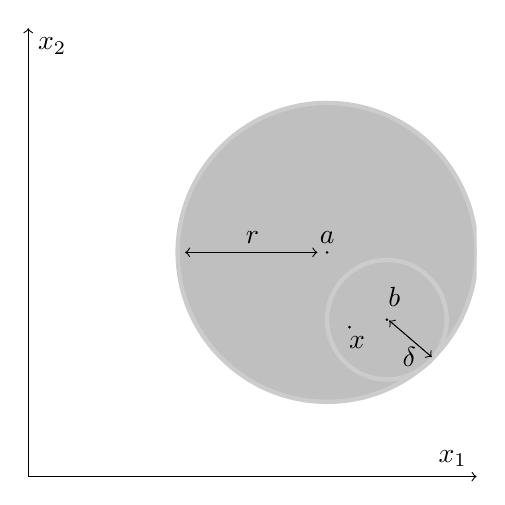
\begin{tikzpicture}
          \begin{axis}[ 
            ticks=none,
            axis lines = middle,
            axis line style={->},
            ymin=0, ymax=3,
            xmin=0, xmax=3,
            xlabel={$x_{1}$},
            ylabel={$x_{2}$},
            axis equal image,
            disabledatascaling
            ]
            \filldraw [ultra thick,fill=black!25!white, draw=black!20!white] (2,1.5) circle [radius=1];
            \filldraw [ultra thick,fill=black!25!white, draw=black!20!white] (2.4,1.05) circle [radius=0.4];
            \fill [fill=black] (2,1.5) circle [radius=0.01];
            \fill [fill=black] (2.4,1.05) circle [radius=0.01];
            \fill [fill=black] (2.15,1) circle [radius=0.01];
            \draw (2,1.6) node {$a$};
            \draw (2.45,1.2) node {$b$};
            \draw (2.2,0.9) node {$x$};
            \draw (2,1.5) node {} edge[<->] (1.05,1.5);
            \draw (1.5,1.6) node {$r$};
            \draw (2.35,1.1) node {} edge[<->] (2.7,0.8);
            \draw (2.55,0.8) node {$\delta$};
          \end{axis}
        \end{tikzpicture}
        \caption{Illustratie in $\mathbb{R}^{2}$}
      \end{figure}
      Kies nu willekeurig een $x\in B(b,\delta)$.
      We tonen aan dat $x$ ook in $B(a,r)$ zit:
      \[ \|x-a\| \le \|x-b\|+\|b-a\| < \delta + \|b-a\| = r\]
  \end{proof}
\end{st}

\begin{de}
  We noemen een deelverzameling $B$ van $\mathbb{R}^{p}$ \term{gesloten} als het complement ervan open is.
\end{de}

\begin{st}
  Een gesloten bol in $\mathbb{R}^{p}$ is een open deelverzameling van $\mathbb{R}^{p}$.

  \begin{proof}
    Inderdaad, beschouw de gesloten bol $B\interval{a}{r}$, kies een willekerugie $b\in \mathbb{R}^{p}\setminus B\interval{a}{r}$ en kies $\delta = \|x-a\|-r$.
      \begin{figure}[H]
        \centering
        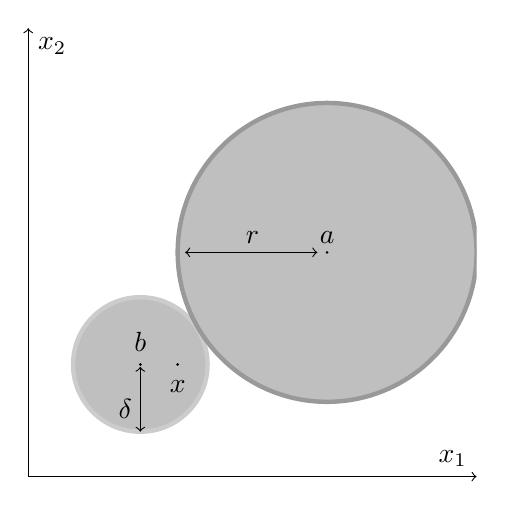
\begin{tikzpicture}
          \begin{axis}[ 
            ticks=none,
            axis lines = middle,
            axis line style={->},
            ymin=0, ymax=3,
            xmin=0, xmax=3,
            xlabel={$x_{1}$},
            ylabel={$x_{2}$},
            axis equal image,
            disabledatascaling
            ]
            \filldraw [ultra thick,fill=black!25!white, draw=black!20!white] (0.75,0.75) circle [radius=0.45];
            \filldraw [ultra thick,fill=black!25!white, draw=black!40!white] (2,1.5) circle [radius=1];
            \fill [fill=black] (2,1.5) circle [radius=0.01];
            \fill [fill=black] (0.75,0.75) circle [radius=0.01];
            \fill [fill=black] (1,0.75) circle [radius=0.01];
            \draw (2,1.6) node {$a$};
            \draw (0.75,0.9) node {$b$};
            \draw (1,0.6) node {$x$};
            \draw (2,1.5) node {} edge[<->] (1.05,1.5);
            \draw (1.5,1.6) node {$r$};
            \draw (0.75,0.8) node {} edge[<->] (0.75,0.3);
            \draw (0.65,0.45) node {$\delta$};
          \end{axis}
        \end{tikzpicture}
        \caption{Illustratie in $\mathbb{R}^{2}$}
      \end{figure}
      Kies nu willekeurig een $x\in B(b,\delta)$.
      We tonen aan dat $x$ ook in $\mathbb{R}^{p}\setminus B\interval{a}{r}$ zit:
      \[ \|b-a\| \le \|b-x\|+\|x-a\| \Rightarrow \delta r+\delta-\delta = r < \|x-a\| \]
  \end{proof}
\end{st}

\begin{vb}
  De verzameling $A$ als volgt is open:
  \[ A = \left\{ x \in \mathbb{R}^{p} \mid \forall i:\ x_{i} \in \interval[open]{-1}{1} \right\} \]

  \begin{proof}
    \begin{figure}[H]
      \centering
      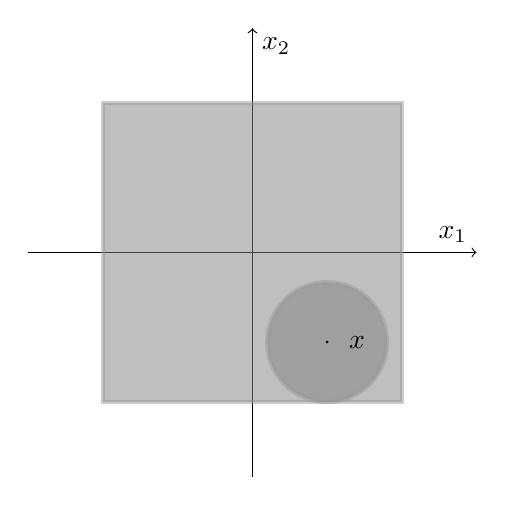
\begin{tikzpicture}
        \begin{axis}[ 
          ticks=none,
          axis lines = middle,
          axis line style={->},
          ymin=-1.5, ymax=1.5,
          xmin=-1.5, xmax=1.5,
          xlabel={$x_{1}$},
          ylabel={$x_{2}$},
          axis equal image,
          disabledatascaling
          ]
          \filldraw [fill=black!50!white, draw=black!40!white,ultra thick,opacity=0.5](-1,-1) rectangle (1,1);
          \filldraw [fill=black!50!white, draw=black!40!white,ultra thick,opacity=0.5] (0.5,-0.6) circle [radius=0.4];
          \fill [fill=black] (0.5,-0.6) circle [radius=0.01];
          \draw (0.7,-0.6) node {$x$};
        \end{axis}
      \end{tikzpicture}
      \caption{Illustratie in $\mathbb{R}^{2}$}
    \end{figure}
    Kies een willekeurige $x\in A$.
    Kies voor $\delta$ het minimum van de volgende verzameling:
    \[ \{ 1-x_{i}\mid i \in \{1,2,\dotsc,p\} \} \cup \{ 1+x_{i}\mid i \in \{1,2,\dotsc,p\} \} \]
    $\delta$ is dan zeker positief.
    Kies nu willekeurig een $y\in B(x,\delta)$, dan moeten we bewijzen dat elke $y_{i}$ strikt tussen $-1$ en $1$ ligt.
    Omdat $y$ in $B(x,\delta)$ zit, geldt $\sqrt{\sum_{i=1}^{p}(x_{i}-p_{i})^{2}} < \delta$.
  \end{proof}
\end{vb}

\begin{vb}
  De verzameling $B$ als volgt is gesloten:
  \[ B = \left\{ x \in \mathbb{R}^{p} \mid \forall i:\ x_{i} \in \interval{-1}{1} \right\} \]

  \begin{proof}
    \begin{figure}[H]
      \centering
      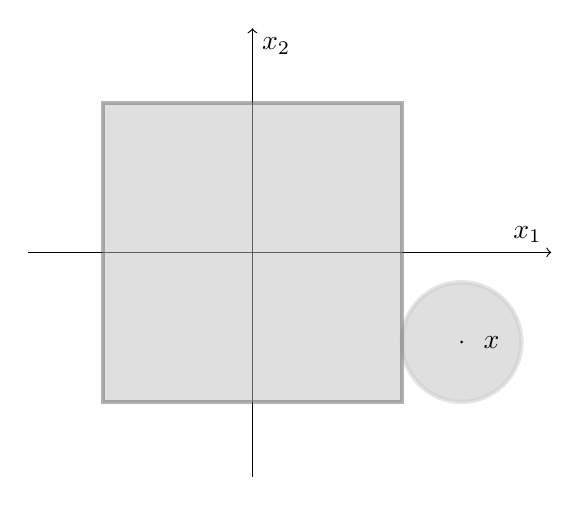
\begin{tikzpicture}
        \begin{axis}[ 
          ticks=none,
          axis lines = middle,
          axis line style={->},
          ymin=-1.5, ymax=1.5,
          xmin=-1.5, xmax=2,
          xlabel={$x_{1}$},
          ylabel={$x_{2}$},
          axis equal image,
          disabledatascaling
          ]
          \filldraw [fill=black!25!white, draw=black!20!white,ultra thick,opacity=0.5] (1.4,-0.6) circle [radius=0.4];
          \filldraw [fill=black!25!white, draw=black!60!white,ultra thick,opacity=0.5](-1,-1) rectangle (1,1);
          
          \fill [fill=black] (1.4,-0.6) circle [radius=0.01];
          \draw (1.6,-0.6) node {$x$};
        \end{axis}
      \end{tikzpicture}
      \caption{Illustratie in $\mathbb{R}^{2}$}
    \end{figure}
    \extra{bewijs}
  \end{proof}
\end{vb}

\begin{vb}
  De verzameling $C$ is noch open, noch gesloten:
  \[ C = \left\{ x \in \mathbb{R}^{p} \mid \forall i:\ x_{i} \in \interval[open left]{-1}{1} \right\} \]
\end{vb}

\begin{pr}
  De unie van open verzamelingen is open.
\extra{bewijs}
\end{pr}

\begin{pr}
  Een eindige doorsnede van open verzamelingen is open.
\extra{bewijs}
\end{pr}

\begin{pr}
  De doorsnede van gesloten verzamelingen is gesloten.
\extra{bewijs}
\end{pr}

\begin{pr}
  Een eindige unie van gesloten verzamelingen is gesloten.
\extra{bewijs}
\end{pr}

\begin{pr}
  Zij $A$ een niet-leeg deel van $\mathbb{R}^{p}$, dan is $A$ gesloten als en slechts als voor elke convergente rij $(x_{n})_{n}$ in $\mathbb{R}^{p}$ de limiet tot $A$ behoort.
\extra{bewijs}
\end{pr}

\begin{st}
  \label{st:in-rp-gesloten-en-begrensd-itv-rijen}
  Zij $A$ een niet-leeg deel van $\mathbb{R}^{p}$, dan is $A$ gesloten en begrensd als en slechts als elke rij in $A$ een convergente deelrij heeft met limiet in $A$.
\extra{bewijs}
\end{st}

\begin{de}
  \label{de:inwendige}
  De grootste open deelverzameling van $A$ noemen we het \term{inwendige} $\mathring{A}$ van $A$.
\end{de}

\begin{de}
  De kleinste gesloten deelverzameling van $A$ noemen we de \term{sluiting} $\overline{A}$ van $A$.
\end{de}

\begin{pr}
  \label{pr:rp-puntsgewijze-karakterisatie-inwendige}
  Zij $A$ een deel van $\mathbb{R}^{p}$, dan kunnen we $\mathring{A}$ als volgt beschrijven:
  \[ \mathring{A} = \{ x \in A \mid \exists \delta \in \mathbb{R}_{0}^{+}:\ B(x,\delta) \subseteq A \} \]
\extra{bewijs}
\end{pr}

\begin{pr}
  \label{pr:rp-puntsgewijze-karakterisatie-sluiting}
  Zij $A$ een deel van $\mathbb{R}^{p}$, dan kunnen we $\overline{A}$ als volgt beschrijven:
  \[ \overline{A} = \{ x \in \mathbb{R}^{p} \mid \forall \delta \in \mathbb{R}_{0}^{+}:\ B(x,\delta) \cap A \neq \emptyset \} \]
\extra{bewijs}
\end{pr}

\begin{pr}
  \label{pr:rp-karakterisatie-sluiting-itv-rijen}
  Zij $A$ een deel van $\mathbb{R}^{p}$ en $x\in \mathbb{R}^{p}$, dan behoort $x$ tot $\overline{A}$ als en slechts als er een rij $(x_{n})_{n}$ in $A$ bestaat met $x$ als limiet.
\extra{bewijs}
\end{pr}

\begin{st}
  Zij $a\in \mathbb{R}^{p}$ en $r\in \mathbb{R}_{0}^{+}$.
  Het inwendige van $B\interval{a}{r}$ is $B(a,r)$.

  \begin{proof}
    Van $B(a,r)$ weten we dat het binnen het inwendige van $B\interval{a}{r}$ ligt (want het is open).\label{de:rp-inwendige}
    Beschouw daarom een punt $x$ dat op een afstand groter dan $r$ ligt van $a$.
    We argumenteren dat $x$ niet in $\mathring{B\interval{a}{r}}$ kan liggen.
    Kies daartoe een willekeurige $\epsilon \in \mathbb{R}_{0}^{+}$ en kies $y=a + (x-a)\left(1+\frac{\epsilon}{\|x-a\|}\right)$.\prref{pr:rp-puntsgewijze-karakterisatie-inwendige}
  \end{proof}
\end{st}

\begin{st}
  Zij $a\in \mathbb{R}^{p}$ en $r\in \mathbb{R}_{0}^{+}$.
  De sluiting van $B(a,r)$ is $B\interval{a}{r}$.

  \begin{proof}
    Van $B(a,r)$ weten we dat het binnen de sluiting ervan ligt.
    Beschouw daarom een punt $x$ dat op een afstand precies $r$ ligt van $a$.
    We zullen een rij contstrueren in $A$ met $x$ als limiet. \prref{pr:rp-karakterisatie-sluiting-itv-rijen}
    Kies daartoe de rij $(a + (r-a)\frac{1}{n})_{n}$.
\question{wat nu?}
  \end{proof}
\end{st}

\begin{de}
  De \term{rand} $\partial A$ van een deelverzameling $A$ van $\mathbb{R}^{+}$ definieren we als volgt:
  \[ \partial A = \overline{A} \setminus \mathring{A} \]
\end{de}

\begin{de}
  Zij $A$ een niet-leeg deel van $\mathbb{R}^{p}$, dan noemen we een punt $x\in A$ een \term{ge\"isoleerd punt} van $A$ als er een $\delta \in \mathbb{R}^{+}$ bestaat als volgt:
  \[ B(x,\delta) \cap A = \{x\} \]
\end{de}

\begin{de}
  Zij $A$ een niet-leeg deel van $\mathbb{R}^{p}$, dan noemen we een punt $x\in A$ een \term{ophopingspunt} van $A$ als voor alle $\delta \in \mathbb{R}^{+}_{0}$ het volgende geldt:
  \[ B(x,\delta) \cap (A \setminus \{x\}) \neq \emptyset \]
\end{de}

\mst{karakterisatie ophopingspunt}

\begin{pr}
  Zij $A$ een niet-leeg deel van $\mathbb{R}^{p}$ en een $x\in \mathbb{R}^{p}$, dan zijn volgende beweringen equivalent:
  \begin{enumerate}
  \item $x$ is een ophopingspunt van $A$.
  \item Voor alle $\delta \in \mathbb{R}_{0}^{+}$, bevat $B(x,\delta) \cap A$ oneindig veel punten.
  \item Er bestaat een rij $(x_{n})_{n}$ in $A\setminus \{ x\}$ die naar $x$ convergeert.
  \end{enumerate}
\extra{bewijs}
\end{pr}


\begin{st}
  De \term{stelling van Bolzano-Weierstra\ss} (ophopingspuntversie)\\
  Elk oneindig, begrensd, deel van $\mathbb{R}^{p}$ heeft minstens \'e\'en ophopingspunt.
\end{st}


\subsection{Relatieve topologie}
\label{sec:relatieve-topologie}

\begin{de}
  Zij $X$ een niet-lege deelverzameling van $\mathbb{R}$.
  We noemen een niet-lege deelverzameling $A$ van $X$ \term{relatief open} in $X$ als het volgende geldt:
  \[ \forall x\in A, \exists \delta \in \mathbb{R}_{0}^{+}, \forall y\in X:\ \|y-x\| < \delta \Rightarrow y \in A \]
\end{de}

\begin{de}
  Zij $X$ een niet-lege deelverzameling van $\mathbb{R}$.
  We noemen een niet-lege deelverzameling $A$ van $X$ \term{relatief open} in $X$ als het relatief complement van $A$ in $X$ relatief open is in $X$.
\end{de}

\begin{pr}
  Zij $X$ een niet-leeg deel van $\mathbb{R}^{p}$ en een $A \subseteq X$, dan is $A$ relatief open in $X$ als en slechts als er een open deel $V$ van $\mathbb{R}^{p}$ bestaat zodat $A$ gelijk is aan $V \cap X$.
\extra{bewijs}
\end{pr}

\begin{pr}
  Zij $X$ een niet-leeg deel van $\mathbb{R}^{p}$ en een $A \subseteq X$, dan is $A$ relatief open in $X$ als en slechts als er een gesloten deel $V$ van $\mathbb{R}^{p}$ bestaat zodat $A$ gelijk is aan $V \cap X$.
\extra{bewijs}
\end{pr}


\end{document}

%%% Local Variables:
%%% mode: latex
%%% TeX-master: t
%%% End:
